\documentclass[tikz,border=6pt]{standalone}
\usepackage[T1]{fontenc}
\usepackage[utf8]{inputenc}
\usepackage{amsmath,amssymb}
\usepackage{tikz}
\usetikzlibrary{automata,positioning,arrows.meta,shapes.geometric,calc,fit}

\tikzset{
    >=Stealth,
    every state/.style={minimum size=8mm, inner sep=1pt, font=\small},
    flow/.style={
        rectangle,
        rounded corners,
        draw,
        align=center,
        minimum width=3.1cm,
        minimum height=0.9cm
    }
}

\begin{document}

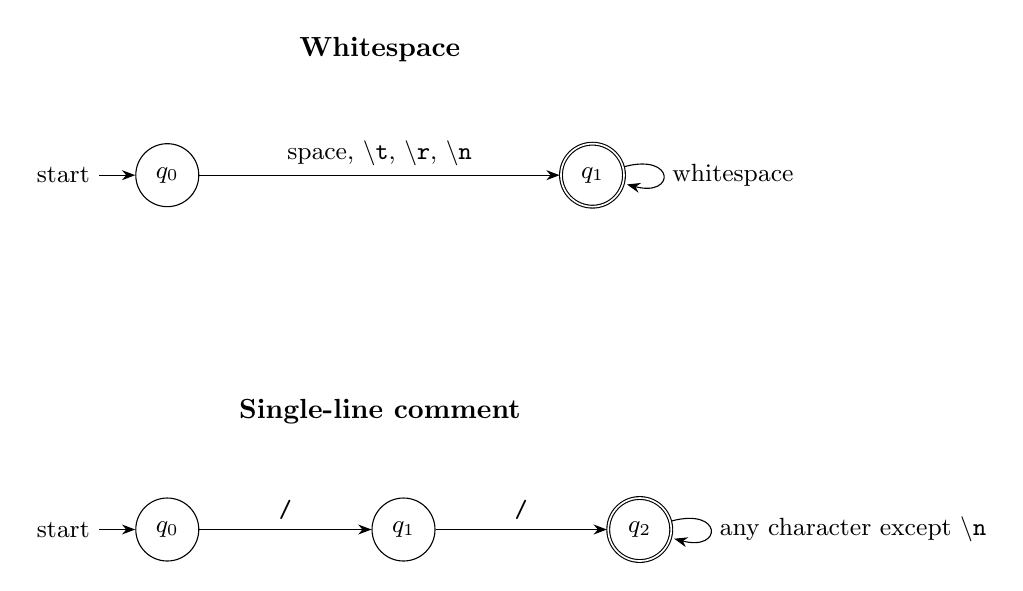
\begin{tikzpicture}[->, font=\small]


\node[font=\bfseries] at (2.7,1.6) {Whitespace};

\node[state, initial] (w0) at (0,0) {$q_0$};
\node[state, accepting] (w1) at (5.4,0) {$q_1$};

\path
    (w0) edge
    node[above] {space, \texttt{\textbackslash t},
                 \texttt{\textbackslash r},
                 \texttt{\textbackslash n}}
    (w1)

    (w1) edge[loop right]
    node[right] {whitespace}
    (w1);


\node[font=\bfseries] at (2.7,-3.0) {Single-line comment};

\node[state, initial] (c0) at (0,-4.5) {$q_0$};
\node[state] (c1) at (3.0,-4.5) {$q_1$};
\node[state, accepting] (c2) at (6.0,-4.5) {$q_2$};

\path
    (c0) edge
    node[above] {\texttt{/}}
    (c1)

    (c1) edge
    node[above] {\texttt{/}}
    (c2)

    (c2) edge[loop right]
    node[right] {any character except \texttt{\textbackslash n}}
    (c2);

\end{tikzpicture}

\end{document}